\documentclass{article}
\usepackage[margin=7mm]{geometry}
\usepackage{tikz}
\usepackage{times}
\usepackage{xcolor}
\usepackage{environ}
\usetikzlibrary{calc}

% Define colors for different sections
\colorlet{stats}{blue!10!white}
\colorlet{proficiencies}{yellow!12!white}
\colorlet{attacks}{orange!25!white}
\colorlet{magic}{red!12!white}
\colorlet{mypurple}{red!40!blue}
\colorlet{features}{magenta!16!white}
\colorlet{playername}{green!90!yellow!8!white}
\colorlet{teal}{blue!40!green}
\colorlet{equipment}{playername}

% Decorative box macro for D&D character sheets
% Usage: \dndbox{x}{y}{width}{height}
% where (x,y) is the lower-left corner
\newcommand{\dndbox}[4]{%
  % Parameters: #1 = x, #2 = y, #3 = width, #4 = height
  \pgfmathsetmacro{\cornersize}{0.15} % Size of corner decorations
  \pgfmathsetmacro{\inset}{0.05} % Inset for inner lines
  
  % Define coordinates
  \coordinate (ll) at (#1, #2);
  \coordinate (lr) at (#1 + #3, #2);
  \coordinate (ul) at (#1, #2 + #4);
  \coordinate (ur) at (#1 + #3, #2 + #4);
  
  % Main outer frame (heavy lines)
  \draw[line width=1.5pt] 
    ($(ll) + (\cornersize, 0)$) -- ($(lr) + (-\cornersize, 0)$)
    ($(lr) + (0, \cornersize)$) -- ($(ur) + (0, -\cornersize)$)
    ($(ur) + (-\cornersize, 0)$) -- ($(ul) + (\cornersize, 0)$)
    ($(ul) + (0, -\cornersize)$) -- ($(ll) + (0, \cornersize)$);
  
  % Corner decorations (ornate corners)
  % Lower-left corner
  \draw[line width=1.5pt] 
    ($(ll) + (\cornersize, 0)$) arc (0:90:\cornersize)
    ($(ll) + (0, \cornersize)$) -- ($(ll) + (0, \cornersize/2)$)
    ($(ll) + (\cornersize, 0)$) -- ($(ll) + (\cornersize/2, 0)$);
  \draw[line width=0.8pt] 
    ($(ll) + (\cornersize*0.7, \cornersize*0.3)$) arc (0:90:\cornersize*0.3);
    
  % Lower-right corner
  \draw[line width=1.5pt] 
    ($(lr) + (-\cornersize, 0)$) arc (180:90:\cornersize)
    ($(lr) + (0, \cornersize)$) -- ($(lr) + (0, \cornersize/2)$)
    ($(lr) + (-\cornersize, 0)$) -- ($(lr) + (-\cornersize/2, 0)$);
  \draw[line width=0.8pt] 
    ($(lr) + (-\cornersize*0.7, \cornersize*0.3)$) arc (180:90:\cornersize*0.3);
    
  % Upper-right corner
  \draw[line width=1.5pt] 
    ($(ur) + (-\cornersize, 0)$) arc (180:270:\cornersize)
    ($(ur) + (0, -\cornersize)$) -- ($(ur) + (0, -\cornersize/2)$)
    ($(ur) + (-\cornersize, 0)$) -- ($(ur) + (-\cornersize/2, 0)$);
  \draw[line width=0.8pt] 
    ($(ur) + (-\cornersize*0.7, -\cornersize*0.3)$) arc (180:270:\cornersize*0.3);
    
  % Upper-left corner
  \draw[line width=1.5pt] 
    ($(ul) + (\cornersize, 0)$) arc (0:-90:\cornersize)
    ($(ul) + (0, -\cornersize)$) -- ($(ul) + (0, -\cornersize/2)$)
    ($(ul) + (\cornersize, 0)$) -- ($(ul) + (\cornersize/2, 0)$);
  \draw[line width=0.8pt] 
    ($(ul) + (\cornersize*0.7, -\cornersize*0.3)$) arc (0:-90:\cornersize*0.3);
  
  % Inner frame lines (lighter)
  \draw[line width=0.5pt]
    ($(ll) + (\inset, \inset)$) rectangle ($(ur) + (-\inset, -\inset)$);
  
  % Double line effect on sides
  \draw[line width=0.3pt]
    ($(ll) + (\inset*2, \cornersize*1.5)$) -- ($(ul) + (\inset*2, -\cornersize*1.5)$)
    ($(lr) + (-\inset*2, \cornersize*1.5)$) -- ($(ur) + (-\inset*2, -\cornersize*1.5)$);
}

% dndsection environment - stores parameters for use inside tikzpicture
\newcommand{\dndsectionx}{}
\newcommand{\dndsectiony}{}
\newcommand{\dndsectionwidth}{}
\newcommand{\dndsectionheight}{}
\newcommand{\dndsectiontitle}{}
\newcommand{\dndsectioncolor}{}

\NewEnviron{dndsection}[6]{%
  \renewcommand{\dndsectionx}{#1}%
  \renewcommand{\dndsectiony}{#2}%
  \renewcommand{\dndsectionwidth}{#3}%
  \renewcommand{\dndsectionheight}{#4}%
  \renewcommand{\dndsectiontitle}{#5}%
  \renewcommand{\dndsectioncolor}{#6}%
  % Fill background
  \fill[\dndsectioncolor] (\dndsectionx + 0.1, \dndsectiony + 0.1) rectangle (\dndsectionx + \dndsectionwidth - 0.1, \dndsectiony + \dndsectionheight - 0.1);
  
  % Draw the decorative box
  \dndbox{\dndsectionx}{\dndsectiony}{\dndsectionwidth}{\dndsectionheight}
  
  % Place the title at the bottom center
  \node[font=\footnotesize\scshape, anchor=south] at (\dndsectionx + \dndsectionwidth/2, \dndsectiony + 0.05) {\sffamily {\dndsectiontitle}};
  
  % Calculate minipage width
  \pgfmathsetmacro{\minipagewidth}{\dndsectionwidth - 0.5}
  
  % Place content in a minipage
  \node[anchor=south west, inner sep=0] at (\dndsectionx + 0.25, \dndsectiony + 0.4) {%
    \begin{minipage}{\minipagewidth cm}%
      \BODY%
    \end{minipage}%
  };
}

\newlength\leftwidth
\newlength\rightwidth
\leftwidth=6.5cm
\rightwidth=12.8cm
\newlength\rightx
\rightx=7.15cm


% Specific section environments with fixed positions
% Use different body names to avoid conflicts
\environbodyname\attacksbody
\NewEnviron{attackssection}{%
  \begin{dndsection}{\rightx}{152mm}{\rightwidth}{48mm}{ATTACKS}{attacks}
    \attacksbody
  \end{dndsection}
}[\ignorespacesafterend]
% y = 128mm for noncasters


\environbodyname\featuresbody

%%\NewEnviron{featuressection}{%  noncaster
%%  \begin{dndsection}{\rightx}{55mm}{\rightwidth}{70mm}{FEATURES}{features}
%%    \featuresbody
%%  \end{dndsection}
%%}[\ignorespacesafterend]
%%

\NewEnviron{featuressection}{%  caster
  \begin{dndsection}{\rightx}{0mm}{\rightwidth}{42mm}{FEATURES}{features}
    \featuresbody
  \end{dndsection}
}[\ignorespacesafterend]


\environbodyname\magicbody  
\NewEnviron{magicsection}{%
  \begin{dndsection}{\rightx}{43mm}{\rightwidth}{105mm}{MAGIC}{magic}
    \magicbody
  \end{dndsection}
}[\ignorespacesafterend]

\environbodyname\equipmentbody
\NewEnviron{equipmentsection}{%
  \begin{dndsection}{0}{0}{68mm}{53mm}{EQUIPMENT}{equipment}
    \equipmentbody
  \end{dndsection}
}[\ignorespacesafterend]

\environbodyname\proficienciesbody
\NewEnviron{proficienciessection}{%
  \begin{dndsection}{30mm}{55mm}{38mm}{160mm}{PROFICIENCIES}{proficiencies}
    \proficienciesbody
  \end{dndsection}
}[\ignorespacesafterend]

\begin{document}
\pagestyle{empty}

\noindent
\begin{tikzpicture}[x=1cm,y=1cm]
  % Set the picture size to text dimensions
  \useasboundingbox (0,0) rectangle (\textwidth,\textheight);
  
  % Equipment section (left side, tall box)
  \begin{equipmentsection}
    \begin{itemize}
      \item Clothes (Fine)
      \item Leather Armor
      \item Shortsword
      \item Lyre
      \item Backpack
      \item Bedroll, Book of Elvish Poetry
      \item Bottle of Ink, Ink Pen
      \item Parchment (10 sheets), Tinderbox
      \item Trail Rations (10 days), Waterskin
    \end{itemize}
  \end{equipmentsection}
  
  % Proficiencies section (middle top)
  \begin{proficienciessection}
    \footnotesize
    \textbf{Acrobatics}\\
    Arcana\\
    History\\
    Investigation\\
    Perception\\
    Performance\\
    Persuasion\\
    Musical Instrument (Lyre)\\
    Language (Common)\\
    Language (Elvish)
  \end{proficienciessection}
  
  % Attacks section (right side, top)
  \begin{attackssection}
    \centering
    \footnotesize
    \begin{tabular}{cccccc}
    \textbf{NAME} & \textbf{ATTACK} & \textbf{DAMAGE} & \textbf{TYPE} & \textbf{RANGE} & \textbf{AMMO}\\
    \hline
    Shortsword & +4 & 1d6+2 & piercing & 5 ft. & ---
    \end{tabular}
  \end{attackssection}
  
  % Magic section (right side, middle)
  \begin{magicsection}
    \footnotesize
    \textbf{NAME}\\[0.2cm]
    Fey Ancestry\\[0.5cm]
    
    \textbf{Bardic Inspiration}\\
    2/day\\[0.5cm]
    
    \textbf{Ritual Caster}
  \end{magicsection}
  
  % Features section (far right)
  \begin{featuressection}
    \footnotesize
    You have advantage to save against charms and you can't be magically put to sleep.\\[0.3cm]
    
    Grant an ally within 60 ft +1d6 inspiration they can use on any one check within 10 minutes.\\[0.3cm]
    
    Cast certain spells as 10-minute rituals instead of using a spell slot.
  \end{featuressection}
\end{tikzpicture}

\end{document}

\documentclass{article}
\usepackage[margin=0pt]{geometry}
\usepackage{tikz}
\usepackage{xcolor}
\usepackage{environ}
\usetikzlibrary{calc}

% Define colors for different sections
\colorlet{stats}{blue!10!white}
\colorlet{proficiencies}{yellow!12!white}
\colorlet{attacks}{orange!25!white}
\colorlet{magic}{red!12!white}
\colorlet{mypurple}{red!40!blue}
\colorlet{features}{magenta!16!white}
\colorlet{playername}{green!90!yellow!8!white}
\colorlet{teal}{blue!40!green}
\colorlet{equipment}{playername}

% Decorative box macro for D&D character sheets
% Usage: \dndbox{x}{y}{width}{height}
% where (x,y) is the lower-left corner
\newcommand{\dndbox}[4]{%
  % Parameters: #1 = x, #2 = y, #3 = width, #4 = height
  \pgfmathsetmacro{\cornersize}{0.15} % Size of corner decorations
  \pgfmathsetmacro{\inset}{0.05} % Inset for inner lines
  
  % Define coordinates
  \coordinate (ll) at (#1, #2);
  \coordinate (lr) at (#1 + #3, #2);
  \coordinate (ul) at (#1, #2 + #4);
  \coordinate (ur) at (#1 + #3, #2 + #4);
  
  % Main outer frame (heavy lines)
  \draw[line width=1.5pt] 
    ($(ll) + (\cornersize, 0)$) -- ($(lr) + (-\cornersize, 0)$)
    ($(lr) + (0, \cornersize)$) -- ($(ur) + (0, -\cornersize)$)
    ($(ur) + (-\cornersize, 0)$) -- ($(ul) + (\cornersize, 0)$)
    ($(ul) + (0, -\cornersize)$) -- ($(ll) + (0, \cornersize)$);
  
  % Corner decorations (ornate corners)
  % Lower-left corner
  \draw[line width=1.5pt] 
    ($(ll) + (\cornersize, 0)$) arc (0:90:\cornersize)
    ($(ll) + (0, \cornersize)$) -- ($(ll) + (0, \cornersize/2)$)
    ($(ll) + (\cornersize, 0)$) -- ($(ll) + (\cornersize/2, 0)$);
  \draw[line width=0.8pt] 
    ($(ll) + (\cornersize*0.7, \cornersize*0.3)$) arc (0:90:\cornersize*0.3);
    
  % Lower-right corner
  \draw[line width=1.5pt] 
    ($(lr) + (-\cornersize, 0)$) arc (180:90:\cornersize)
    ($(lr) + (0, \cornersize)$) -- ($(lr) + (0, \cornersize/2)$)
    ($(lr) + (-\cornersize, 0)$) -- ($(lr) + (-\cornersize/2, 0)$);
  \draw[line width=0.8pt] 
    ($(lr) + (-\cornersize*0.7, \cornersize*0.3)$) arc (180:90:\cornersize*0.3);
    
  % Upper-right corner
  \draw[line width=1.5pt] 
    ($(ur) + (-\cornersize, 0)$) arc (180:270:\cornersize)
    ($(ur) + (0, -\cornersize)$) -- ($(ur) + (0, -\cornersize/2)$)
    ($(ur) + (-\cornersize, 0)$) -- ($(ur) + (-\cornersize/2, 0)$);
  \draw[line width=0.8pt] 
    ($(ur) + (-\cornersize*0.7, -\cornersize*0.3)$) arc (180:270:\cornersize*0.3);
    
  % Upper-left corner
  \draw[line width=1.5pt] 
    ($(ul) + (\cornersize, 0)$) arc (0:-90:\cornersize)
    ($(ul) + (0, -\cornersize)$) -- ($(ul) + (0, -\cornersize/2)$)
    ($(ul) + (\cornersize, 0)$) -- ($(ul) + (\cornersize/2, 0)$);
  \draw[line width=0.8pt] 
    ($(ul) + (\cornersize*0.7, -\cornersize*0.3)$) arc (0:-90:\cornersize*0.3);
  
  % Inner frame lines (lighter)
  \draw[line width=0.5pt]
    ($(ll) + (\inset, \inset)$) rectangle ($(ur) + (-\inset, -\inset)$);
  
  % Double line effect on sides
  \draw[line width=0.3pt]
    ($(ll) + (\inset*2, \cornersize*1.5)$) -- ($(ul) + (\inset*2, -\cornersize*1.5)$)
    ($(lr) + (-\inset*2, \cornersize*1.5)$) -- ($(ur) + (-\inset*2, -\cornersize*1.5)$);
}

% dndsection environment - stores parameters for use inside tikzpicture
\newcommand{\dndsectionx}{}
\newcommand{\dndsectiony}{}
\newcommand{\dndsectionwidth}{}
\newcommand{\dndsectionheight}{}
\newcommand{\dndsectiontitle}{}
\newcommand{\dndsectioncolor}{}

\NewEnviron{dndsection}[6]{%
  \renewcommand{\dndsectionx}{#1}%
  \renewcommand{\dndsectiony}{#2}%
  \renewcommand{\dndsectionwidth}{#3}%
  \renewcommand{\dndsectionheight}{#4}%
  \renewcommand{\dndsectiontitle}{#5}%
  \renewcommand{\dndsectioncolor}{#6}%
  % Fill background
  \fill[\dndsectioncolor] (\dndsectionx + 0.1, \dndsectiony + 0.1) rectangle (\dndsectionx + \dndsectionwidth - 0.1, \dndsectiony + \dndsectionheight - 0.1);
  
  % Draw the decorative box
  \dndbox{\dndsectionx}{\dndsectiony}{\dndsectionwidth}{\dndsectionheight}
  
  % Place the title at the bottom center
  \node[font=\footnotesize\scshape, anchor=south] at (\dndsectionx + \dndsectionwidth/2, \dndsectiony + 0.05) {\dndsectiontitle};
  
  % Calculate minipage width
  \pgfmathsetmacro{\minipagewidth}{\dndsectionwidth - 0.5}
  
  % Place content in a minipage
  \node[anchor=south west, inner sep=0] at (\dndsectionx + 0.25, \dndsectiony + 0.4) {%
    \begin{minipage}{\minipagewidth cm}%
      \BODY%
    \end{minipage}%
  };
}

% Specific section environments with fixed positions
% Use different body names to avoid conflicts
\environbodyname\attacksbody
\NewEnviron{attackssection}{%
  \begin{dndsection}{10.5}{18.5}{10}{4.5}{ATTACKS}{attacks}
    \attacksbody
  \end{dndsection}
}[\ignorespacesafterend]

\environbodyname\magicbody  
\NewEnviron{magicsection}{%
  \begin{dndsection}{10.5}{13.5}{10}{4.5}{MAGIC}{magic}
    \magicbody
  \end{dndsection}
}[\ignorespacesafterend]

\environbodyname\featuresbody
\NewEnviron{featuressection}{%
  \begin{dndsection}{10.5}{23.5}{10}{3.5}{FEATURES}{features}
    \featuresbody
  \end{dndsection}
}[\ignorespacesafterend]

\environbodyname\equipmentbody
\NewEnviron{equipmentsection}{%
  \begin{dndsection}{0.5}{13.5}{9.5}{9.5}{EQUIPMENT}{equipment}
    \equipmentbody
  \end{dndsection}
}[\ignorespacesafterend]

\environbodyname\proficienciesbody
\NewEnviron{proficienciessection}{%
  \begin{dndsection}{0.5}{23.5}{9.5}{3.5}{PROFICIENCIES}{proficiencies}
    \proficienciesbody
  \end{dndsection}
}[\ignorespacesafterend]

\begin{document}
\pagestyle{empty}

% Set document to US Letter size
\pdfpagewidth=8.5in
\pdfpageheight=11in

\begin{tikzpicture}[remember picture]
  % Shift origin to bottom-left of page
  \coordinate (origin) at (current page.south west);
  
  % Equipment section (left side, tall box)
  \begin{equipmentsection}
    \begin{itemize}
      \item Clothes (Fine)
      \item Leather Armor
      \item Shortsword
      \item Lyre
      \item Backpack
      \item Bedroll, Book of Elvish Poetry
      \item Bottle of Ink, Ink Pen
      \item Parchment (10 sheets), Tinderbox
      \item Trail Rations (10 days), Waterskin
    \end{itemize}
  \end{equipmentsection}
  
  % Proficiencies section (left side, top)
  \begin{proficienciessection}
    \textbf{Armor:} Light armor\\
    \textbf{Weapons:} Simple weapons, hand crossbows, longswords, rapiers, shortswords\\
    \textbf{Tools:} Three musical instruments (Lyre, Flute, Drums)\\
    \textbf{Saving Throws:} Dexterity, Charisma\\
    \textbf{Skills:} Acrobatics, Arcana, History, Insight, Investigation, Perception, Performance, Persuasion\\
    \textbf{Languages:} Common, Elvish
  \end{proficienciessection}
  
  % Attacks section (right side, middle)
  \begin{attackssection}
    \textbf{NAME \hfill ATTACK \hfill DAMAGE \hfill TYPE \hfill RANGE \hfill AMMO}\\
    \rule{\linewidth}{0.4pt}\\
    Shortsword \hfill +4 \hfill 1d6+2 \hfill piercing \hfill 5 ft. \hfill ---
  \end{attackssection}
  
  % Magic section (right side, bottom)
  \begin{magicsection}
    \textbf{NAME}\\
    Fey Ancestry\\[0.3cm]
    \textbf{Bardic Inspiration}\\
    2/day\\[0.3cm]
    \textbf{Ritual Caster}
  \end{magicsection}
  
  % Features section (right side, top)
  \begin{featuressection}
    You have advantage to save against charms and you can't be magically put to sleep.\\[0.3cm]
    Grant an ally within 60 ft +1d6 inspiration they can use on any one check within 10 minutes.\\[0.3cm]
    Cast certain spells as 10-minute rituals instead of using a spell slot.
  \end{featuressection}
\end{tikzpicture}

\end{document}


\documentclass{article}
\usepackage{tikz}
\usepackage{xcolor}
\usepackage{environ}
\usetikzlibrary{calc}

% Define colors for different sections
\colorlet{stats}{blue!10!white}
\colorlet{proficiencies}{yellow!12!white}
\colorlet{attacks}{orange!25!white}
\colorlet{magic}{red!12!white}
\colorlet{mypurple}{red!40!blue}
\colorlet{features}{magenta!16!white}
\colorlet{playername}{green!90!yellow!8!white}
\colorlet{teal}{blue!40!green}
\colorlet{equipment}{playername}

% Decorative box macro for D&D character sheets
% Usage: \dndbox{x}{y}{width}{height}
% where (x,y) is the lower-left corner
\newcommand{\dndbox}[4]{%
  % Parameters: #1 = x, #2 = y, #3 = width, #4 = height
  \pgfmathsetmacro{\cornersize}{0.15} % Size of corner decorations
  \pgfmathsetmacro{\inset}{0.05} % Inset for inner lines
  
  % Define coordinates
  \coordinate (ll) at (#1, #2);
  \coordinate (lr) at (#1 + #3, #2);
  \coordinate (ul) at (#1, #2 + #4);
  \coordinate (ur) at (#1 + #3, #2 + #4);
  
  % Main outer frame (heavy lines)
  \draw[line width=1.5pt] 
    ($(ll) + (\cornersize, 0)$) -- ($(lr) + (-\cornersize, 0)$)
    ($(lr) + (0, \cornersize)$) -- ($(ur) + (0, -\cornersize)$)
    ($(ur) + (-\cornersize, 0)$) -- ($(ul) + (\cornersize, 0)$)
    ($(ul) + (0, -\cornersize)$) -- ($(ll) + (0, \cornersize)$);
  
  % Corner decorations (ornate corners)
  % Lower-left corner
  \draw[line width=1.5pt] 
    ($(ll) + (\cornersize, 0)$) arc (0:90:\cornersize)
    ($(ll) + (0, \cornersize)$) -- ($(ll) + (0, \cornersize/2)$)
    ($(ll) + (\cornersize, 0)$) -- ($(ll) + (\cornersize/2, 0)$);
  \draw[line width=0.8pt] 
    ($(ll) + (\cornersize*0.7, \cornersize*0.3)$) arc (0:90:\cornersize*0.3);
    
  % Lower-right corner
  \draw[line width=1.5pt] 
    ($(lr) + (-\cornersize, 0)$) arc (180:90:\cornersize)
    ($(lr) + (0, \cornersize)$) -- ($(lr) + (0, \cornersize/2)$)
    ($(lr) + (-\cornersize, 0)$) -- ($(lr) + (-\cornersize/2, 0)$);
  \draw[line width=0.8pt] 
    ($(lr) + (-\cornersize*0.7, \cornersize*0.3)$) arc (180:90:\cornersize*0.3);
    
  % Upper-right corner
  \draw[line width=1.5pt] 
    ($(ur) + (-\cornersize, 0)$) arc (180:270:\cornersize)
    ($(ur) + (0, -\cornersize)$) -- ($(ur) + (0, -\cornersize/2)$)
    ($(ur) + (-\cornersize, 0)$) -- ($(ur) + (-\cornersize/2, 0)$);
  \draw[line width=0.8pt] 
    ($(ur) + (-\cornersize*0.7, -\cornersize*0.3)$) arc (180:270:\cornersize*0.3);
    
  % Upper-left corner
  \draw[line width=1.5pt] 
    ($(ul) + (\cornersize, 0)$) arc (0:-90:\cornersize)
    ($(ul) + (0, -\cornersize)$) -- ($(ul) + (0, -\cornersize/2)$)
    ($(ul) + (\cornersize, 0)$) -- ($(ul) + (\cornersize/2, 0)$);
  \draw[line width=0.8pt] 
    ($(ul) + (\cornersize*0.7, -\cornersize*0.3)$) arc (0:-90:\cornersize*0.3);
  
  % Inner frame lines (lighter)
  \draw[line width=0.5pt]
    ($(ll) + (\inset, \inset)$) rectangle ($(ur) + (-\inset, -\inset)$);
  
  % Double line effect on sides
  \draw[line width=0.3pt]
    ($(ll) + (\inset*2, \cornersize*1.5)$) -- ($(ul) + (\inset*2, -\cornersize*1.5)$)
    ($(lr) + (-\inset*2, \cornersize*1.5)$) -- ($(ur) + (-\inset*2, -\cornersize*1.5)$);
}

% dndsection environment - stores parameters for use inside tikzpicture
\newcommand{\dndsectionx}{}
\newcommand{\dndsectiony}{}
\newcommand{\dndsectionwidth}{}
\newcommand{\dndsectionheight}{}
\newcommand{\dndsectiontitle}{}
\newcommand{\dndsectioncolor}{}

\NewEnviron{dndsection}[6]{%
  \renewcommand{\dndsectionx}{#1}%
  \renewcommand{\dndsectiony}{#2}%
  \renewcommand{\dndsectionwidth}{#3}%
  \renewcommand{\dndsectionheight}{#4}%
  \renewcommand{\dndsectiontitle}{#5}%
  \renewcommand{\dndsectioncolor}{#6}%
  % Fill background
  \fill[\dndsectioncolor] (\dndsectionx + 0.1, \dndsectiony + 0.1) rectangle (\dndsectionx + \dndsectionwidth - 0.1, \dndsectiony + \dndsectionheight - 0.1);
  
  % Draw the decorative box
  \dndbox{\dndsectionx}{\dndsectiony}{\dndsectionwidth}{\dndsectionheight}
  
  % Place the title at the bottom center
  \node[font=\footnotesize\scshape, anchor=south] at (\dndsectionx + \dndsectionwidth/2, \dndsectiony + 0.05) {\dndsectiontitle};
  
  % Calculate minipage width
  \pgfmathsetmacro{\minipagewidth}{\dndsectionwidth - 0.5}
  
  % Place content in a minipage
  \node[anchor=south west, inner sep=0] at (\dndsectionx + 0.25, \dndsectiony + 0.4) {%
    \begin{minipage}{\minipagewidth cm}%
      \BODY%
    \end{minipage}%
  };
}

% Specific section environments with fixed positions
% Use different body names to avoid conflicts
\environbodyname\attacksbody
\NewEnviron{attackssection}{%
  \begin{dndsection}{8.5}{4.5}{5.5}{2.8}{ATTACKS}{attacks}
    \attacksbody
  \end{dndsection}
}[\ignorespacesafterend]

\environbodyname\magicbody  
\NewEnviron{magicsection}{%
  \begin{dndsection}{8.5}{0.5}{5.5}{3.8}{MAGIC}{magic}
    \magicbody
  \end{dndsection}
}[\ignorespacesafterend]

\environbodyname\featuresbody
\NewEnviron{featuressection}{%
  \begin{dndsection}{14.2}{0.5}{5.5}{3}{FEATURES}{features}
    \featuresbody
  \end{dndsection}
}[\ignorespacesafterend]

\environbodyname\equipmentbody
\NewEnviron{equipmentsection}{%
  \begin{dndsection}{0.5}{0.5}{4}{6.5}{EQUIPMENT}{equipment}
    \equipmentbody
  \end{dndsection}
}[\ignorespacesafterend]

\environbodyname\proficienciesbody
\NewEnviron{proficienciessection}{%
  \begin{dndsection}{4.7}{4.5}{3.6}{2.8}{PROFICIENCIES}{proficiencies}
    \proficienciesbody
  \end{dndsection}
}[\ignorespacesafterend]

\begin{document}
\pagestyle{empty}

\begin{tikzpicture}[remember picture, overlay]
  % Current page node gives us the page dimensions
  \coordinate (page) at (current page.south west);
  
  % Equipment section (left side)
  \begin{equipmentsection}
    \begin{itemize}
      \item Clothes (Fine)
      \item Leather Armor
      \item Shortsword
      \item Lyre
      \item Backpack
      \item Bedroll, Book of Elvish Poetry
      \item Bottle of Ink, Ink Pen
      \item Parchment (10 sheets), Tinderbox
      \item Trail Rations (10 days), Waterskin
    \end{itemize}
  \end{equipmentsection}
  
  % Proficiencies section (middle)
  \begin{proficienciessection}
    \textbf{Armor:} Light armor\\
    \textbf{Weapons:} Simple weapons, hand crossbows, longswords, rapiers, shortswords\\
    \textbf{Tools:} Lyre, Flute, Drums\\
    \textbf{Languages:} Common, Elvish
  \end{proficienciessection}
  
  % Attacks section (upper right)
  \begin{attackssection}
    \textbf{Shortsword}\\
    \textit{Melee Weapon Attack:} +4 to hit, reach 5 ft., one target.\\
    \textit{Hit:} 1d6+2 piercing damage.
  \end{attackssection}
  
  % Magic section (lower right)
  \begin{magicsection}
    \textbf{Fey Ancestry}\\
    You have advantage to save against charms and you can't be magically put to sleep.
    
    \vspace{0.2cm}
    \textbf{Bardic Inspiration (2/day)}\\
    Grant an ally within 60 ft +1d6 inspiration they can use on any one check within 10 minutes.
  \end{magicsection}
  
  % Features section (far right)
  \begin{featuressection}
    \textbf{Darkvision (60 ft.)}\\
    You can see in dim light as if it were bright light.
    
    \vspace{0.2cm}
    \textbf{Trance}\\
    Elves meditate deeply for 4 hours a day.
  \end{featuressection}
\end{tikzpicture}

\end{document}

\documentclass{article}
\usepackage{tikz}
\usepackage{xcolor}
\usepackage{environ}
\usetikzlibrary{calc}

% Define colors for different sections
\colorlet{stats}{blue!10!white}
\colorlet{proficiencies}{yellow!12!white}
\colorlet{attacks}{orange!25!white}
\colorlet{magic}{red!12!white}
\colorlet{mypurple}{red!40!blue}
\colorlet{features}{magenta!16!white}
\colorlet{playername}{green!90!yellow!8!white}
\colorlet{teal}{blue!40!green}
\colorlet{equipment}{playername}

% Decorative box macro for D&D character sheets
% Usage: \dndbox{x}{y}{width}{height}
% where (x,y) is the lower-left corner
\newcommand{\dndbox}[4]{%
  % Parameters: #1 = x, #2 = y, #3 = width, #4 = height
  \pgfmathsetmacro{\cornersize}{0.15} % Size of corner decorations
  \pgfmathsetmacro{\inset}{0.05} % Inset for inner lines
  
  % Define coordinates
  \coordinate (ll) at (#1, #2);
  \coordinate (lr) at (#1 + #3, #2);
  \coordinate (ul) at (#1, #2 + #4);
  \coordinate (ur) at (#1 + #3, #2 + #4);
  
  % Main outer frame (heavy lines)
  \draw[line width=1.5pt] 
    ($(ll) + (\cornersize, 0)$) -- ($(lr) + (-\cornersize, 0)$)
    ($(lr) + (0, \cornersize)$) -- ($(ur) + (0, -\cornersize)$)
    ($(ur) + (-\cornersize, 0)$) -- ($(ul) + (\cornersize, 0)$)
    ($(ul) + (0, -\cornersize)$) -- ($(ll) + (0, \cornersize)$);
  
  % Corner decorations (ornate corners)
  % Lower-left corner
  \draw[line width=1.5pt] 
    ($(ll) + (\cornersize, 0)$) arc (0:90:\cornersize)
    ($(ll) + (0, \cornersize)$) -- ($(ll) + (0, \cornersize/2)$)
    ($(ll) + (\cornersize, 0)$) -- ($(ll) + (\cornersize/2, 0)$);
  \draw[line width=0.8pt] 
    ($(ll) + (\cornersize*0.7, \cornersize*0.3)$) arc (0:90:\cornersize*0.3);
    
  % Lower-right corner
  \draw[line width=1.5pt] 
    ($(lr) + (-\cornersize, 0)$) arc (180:90:\cornersize)
    ($(lr) + (0, \cornersize)$) -- ($(lr) + (0, \cornersize/2)$)
    ($(lr) + (-\cornersize, 0)$) -- ($(lr) + (-\cornersize/2, 0)$);
  \draw[line width=0.8pt] 
    ($(lr) + (-\cornersize*0.7, \cornersize*0.3)$) arc (180:90:\cornersize*0.3);
    
  % Upper-right corner
  \draw[line width=1.5pt] 
    ($(ur) + (-\cornersize, 0)$) arc (180:270:\cornersize)
    ($(ur) + (0, -\cornersize)$) -- ($(ur) + (0, -\cornersize/2)$)
    ($(ur) + (-\cornersize, 0)$) -- ($(ur) + (-\cornersize/2, 0)$);
  \draw[line width=0.8pt] 
    ($(ur) + (-\cornersize*0.7, -\cornersize*0.3)$) arc (180:270:\cornersize*0.3);
    
  % Upper-left corner
  \draw[line width=1.5pt] 
    ($(ul) + (\cornersize, 0)$) arc (0:-90:\cornersize)
    ($(ul) + (0, -\cornersize)$) -- ($(ul) + (0, -\cornersize/2)$)
    ($(ul) + (\cornersize, 0)$) -- ($(ul) + (\cornersize/2, 0)$);
  \draw[line width=0.8pt] 
    ($(ul) + (\cornersize*0.7, -\cornersize*0.3)$) arc (0:-90:\cornersize*0.3);
  
  % Inner frame lines (lighter)
  \draw[line width=0.5pt]
    ($(ll) + (\inset, \inset)$) rectangle ($(ur) + (-\inset, -\inset)$);
  
  % Double line effect on sides
  \draw[line width=0.3pt]
    ($(ll) + (\inset*2, \cornersize*1.5)$) -- ($(ul) + (\inset*2, -\cornersize*1.5)$)
    ($(lr) + (-\inset*2, \cornersize*1.5)$) -- ($(ur) + (-\inset*2, -\cornersize*1.5)$);
}

% dndsection environment - stores parameters for use inside tikzpicture
\newcommand{\dndsectionx}{}
\newcommand{\dndsectiony}{}
\newcommand{\dndsectionwidth}{}
\newcommand{\dndsectionheight}{}
\newcommand{\dndsectiontitle}{}
\newcommand{\dndsectioncolor}{}

\NewEnviron{dndsection}[6]{%
  \renewcommand{\dndsectionx}{#1}%
  \renewcommand{\dndsectiony}{#2}%
  \renewcommand{\dndsectionwidth}{#3}%
  \renewcommand{\dndsectionheight}{#4}%
  \renewcommand{\dndsectiontitle}{#5}%
  \renewcommand{\dndsectioncolor}{#6}%
  % Fill background
  \fill[\dndsectioncolor] (\dndsectionx + 0.1, \dndsectiony + 0.1) rectangle (\dndsectionx + \dndsectionwidth - 0.1, \dndsectiony + \dndsectionheight - 0.1);
  
  % Draw the decorative box
  \dndbox{\dndsectionx}{\dndsectiony}{\dndsectionwidth}{\dndsectionheight}
  
  % Place the title at the bottom center
  \node[font=\footnotesize\scshape, anchor=south] at (\dndsectionx + \dndsectionwidth/2, \dndsectiony + 0.05) {\dndsectiontitle};
  
  % Calculate minipage width
  \pgfmathsetmacro{\minipagewidth}{\dndsectionwidth - 0.5}
  
  % Place content in a minipage
  \node[anchor=south west, inner sep=0] at (\dndsectionx + 0.25, \dndsectiony + 0.4) {%
    \begin{minipage}{\minipagewidth cm}%
      ZORCH%
    \end{minipage}%
  };
}

\begin{document}
\pagestyle{empty}

\begin{tikzpicture}[remember picture, overlay]
  % Current page node gives us the page dimensions
  \coordinate (page) at (current page.south west);
  
  % Equipment section (left side)
  \begin{equipmentsection}
    \begin{itemize}
      \item Clothes (Fine)
      \item Leather Armor
      \item Shortsword
      \item Lyre
      \item Backpack
      \item Bedroll, Book of Elvish Poetry
      \item Bottle of Ink, Ink Pen
      \item Parchment (10 sheets), Tinderbox
      \item Trail Rations (10 days), Waterskin
    \end{itemize}
  \end{equipmentsection}
  
  % Proficiencies section (middle)
  \begin{proficienciessection}
    \textbf{Armor:} Light armor\\
    \textbf{Weapons:} Simple weapons, hand crossbows, longswords, rapiers, shortswords\\
    \textbf{Tools:} Lyre, Flute, Drums\\
    \textbf{Languages:} Common, Elvish
  \end{proficienciessection}
  
  % Attacks section (upper right)
  \begin{attackssection}
    \textbf{Shortsword}\\
    \textit{Melee Weapon Attack:} +4 to hit, reach 5 ft., one target.\\
    \textit{Hit:} 1d6+2 piercing damage.
  \end{attackssection}
  
  % Magic section (lower right)
  \begin{magicsection}
    \textbf{Fey Ancestry}\\
    You have advantage to save against charms and you can't be magically put to sleep.
    
    \vspace{0.2cm}
    \textbf{Bardic Inspiration (2/day)}\\
    Grant an ally within 60 ft +1d6 inspiration they can use on any one check within 10 minutes.
  \end{magicsection}
  
  % Features section (far right)
  \begin{featuressection}
    \textbf{Darkvision (60 ft.)}\\
    You can see in dim light as if it were bright light.
    
    \vspace{0.2cm}
    \textbf{Trance}\\
    Elves meditate deeply for 4 hours a day.
  \end{featuressection}
\end{tikzpicture}

\end{document}

\documentclass{article}
\usepackage{tikz}
\usepackage{xcolor}
\usepackage{environ}
\usetikzlibrary{calc}

% Define colors for different sections
\colorlet{stats}{blue!10!white}
\colorlet{proficiencies}{yellow!12!white}
\colorlet{attacks}{orange!25!white}
\colorlet{magic}{red!12!white}
\colorlet{mypurple}{red!40!blue}
\colorlet{features}{magenta!16!white}
\colorlet{playername}{green!90!yellow!8!white}
\colorlet{teal}{blue!40!green}
\colorlet{equipment}{playername}

% Decorative box macro for D&D character sheets
% Usage: \dndbox{x}{y}{width}{height}
% where (x,y) is the lower-left corner
\newcommand{\dndbox}[4]{%
  % Parameters: #1 = x, #2 = y, #3 = width, #4 = height
  \pgfmathsetmacro{\cornersize}{0.15} % Size of corner decorations
  \pgfmathsetmacro{\inset}{0.05} % Inset for inner lines
  
  % Define coordinates
  \coordinate (ll) at (#1, #2);
  \coordinate (lr) at (#1 + #3, #2);
  \coordinate (ul) at (#1, #2 + #4);
  \coordinate (ur) at (#1 + #3, #2 + #4);
  
  % Main outer frame (heavy lines)
  \draw[line width=1.5pt] 
    ($(ll) + (\cornersize, 0)$) -- ($(lr) + (-\cornersize, 0)$)
    ($(lr) + (0, \cornersize)$) -- ($(ur) + (0, -\cornersize)$)
    ($(ur) + (-\cornersize, 0)$) -- ($(ul) + (\cornersize, 0)$)
    ($(ul) + (0, -\cornersize)$) -- ($(ll) + (0, \cornersize)$);
  
  % Corner decorations (ornate corners)
  % Lower-left corner
  \draw[line width=1.5pt] 
    ($(ll) + (\cornersize, 0)$) arc (0:90:\cornersize)
    ($(ll) + (0, \cornersize)$) -- ($(ll) + (0, \cornersize/2)$)
    ($(ll) + (\cornersize, 0)$) -- ($(ll) + (\cornersize/2, 0)$);
  \draw[line width=0.8pt] 
    ($(ll) + (\cornersize*0.7, \cornersize*0.3)$) arc (0:90:\cornersize*0.3);
    
  % Lower-right corner
  \draw[line width=1.5pt] 
    ($(lr) + (-\cornersize, 0)$) arc (180:90:\cornersize)
    ($(lr) + (0, \cornersize)$) -- ($(lr) + (0, \cornersize/2)$)
    ($(lr) + (-\cornersize, 0)$) -- ($(lr) + (-\cornersize/2, 0)$);
  \draw[line width=0.8pt] 
    ($(lr) + (-\cornersize*0.7, \cornersize*0.3)$) arc (180:90:\cornersize*0.3);
    
  % Upper-right corner
  \draw[line width=1.5pt] 
    ($(ur) + (-\cornersize, 0)$) arc (180:270:\cornersize)
    ($(ur) + (0, -\cornersize)$) -- ($(ur) + (0, -\cornersize/2)$)
    ($(ur) + (-\cornersize, 0)$) -- ($(ur) + (-\cornersize/2, 0)$);
  \draw[line width=0.8pt] 
    ($(ur) + (-\cornersize*0.7, -\cornersize*0.3)$) arc (180:270:\cornersize*0.3);
    
  % Upper-left corner
  \draw[line width=1.5pt] 
    ($(ul) + (\cornersize, 0)$) arc (0:-90:\cornersize)
    ($(ul) + (0, -\cornersize)$) -- ($(ul) + (0, -\cornersize/2)$)
    ($(ul) + (\cornersize, 0)$) -- ($(ul) + (\cornersize/2, 0)$);
  \draw[line width=0.8pt] 
    ($(ul) + (\cornersize*0.7, -\cornersize*0.3)$) arc (0:-90:\cornersize*0.3);
  
  % Inner frame lines (lighter)
  \draw[line width=0.5pt]
    ($(ll) + (\inset, \inset)$) rectangle ($(ur) + (-\inset, -\inset)$);
  
  % Double line effect on sides
  \draw[line width=0.3pt]
    ($(ll) + (\inset*2, \cornersize*1.5)$) -- ($(ul) + (\inset*2, -\cornersize*1.5)$)
    ($(lr) + (-\inset*2, \cornersize*1.5)$) -- ($(ur) + (-\inset*2, -\cornersize*1.5)$);
}

% dndsection environment - stores parameters for use inside tikzpicture
\newcommand{\dndsectionx}{}
\newcommand{\dndsectiony}{}
\newcommand{\dndsectionwidth}{}
\newcommand{\dndsectionheight}{}
\newcommand{\dndsectiontitle}{}
\newcommand{\dndsectioncolor}{}

\NewEnviron{dndsection}[6]{%
  \renewcommand{\dndsectionx}{#1}%
  \renewcommand{\dndsectiony}{#2}%
  \renewcommand{\dndsectionwidth}{#3}%
  \renewcommand{\dndsectionheight}{#4}%
  \renewcommand{\dndsectiontitle}{#5}%
  \renewcommand{\dndsectioncolor}{#6}%
  % Fill background
  \fill[\dndsectioncolor] (\dndsectionx + 0.1, \dndsectiony + 0.1) rectangle (\dndsectionx + \dndsectionwidth - 0.1, \dndsectiony + \dndsectionheight - 0.1);
  
  % Draw the decorative box
  \dndbox{\dndsectionx}{\dndsectiony}{\dndsectionwidth}{\dndsectionheight}
  
  % Place the title at the bottom center
  \node[font=\footnotesize\scshape, anchor=south] at (\dndsectionx + \dndsectionwidth/2, \dndsectiony + 0.05) {\dndsectiontitle};
  
  % Calculate minipage width
  \pgfmathsetmacro{\minipagewidth}{\dndsectionwidth - 0.5}
  
  % Place content in a minipage
  \node[anchor=south west, inner sep=0] at (\dndsectionx + 0.25, \dndsectiony + 0.4) {%
    \begin{minipage}{\minipagewidth cm}%
      \BODY%
    \end{minipage}%
  };
}

\begin{document}
\pagestyle{empty}

% Test 1: Basic tikzpicture without overlay
\begin{tikzpicture}
  % Simple test with just dndsection
  \begin{dndsection}{0}{0}{6}{3}{TEST SECTION}{attacks}
    This content will be ignored and replaced with ZORCH
  \end{dndsection}
\end{tikzpicture}

\vspace{1cm}

% Test 2: Even simpler - just the box
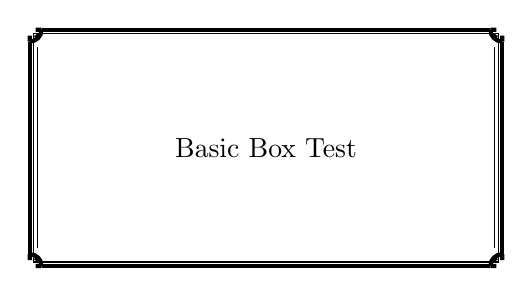
\begin{tikzpicture}
  \dndbox{0}{0}{6}{3}
  \node at (3,1.5) {Basic Box Test};
\end{tikzpicture}

\end{document}

\documentclass{article}
\usepackage{tikz}
\usepackage{xcolor}
\usepackage{environ}
\usetikzlibrary{calc}

% Define colors for different sections
\colorlet{stats}{blue!10!white}
\colorlet{proficiencies}{yellow!12!white}
\colorlet{attacks}{orange!25!white}
\colorlet{magic}{red!12!white}
\colorlet{mypurple}{red!40!blue}
\colorlet{features}{magenta!16!white}
\colorlet{playername}{green!90!yellow!8!white}
\colorlet{teal}{blue!40!green}
\colorlet{equipment}{playername}

% Decorative box macro for D&D character sheets
% Usage: \dndbox{x}{y}{width}{height}
% where (x,y) is the lower-left corner
\newcommand{\dndbox}[4]{%
  % Parameters: #1 = x, #2 = y, #3 = width, #4 = height
  \pgfmathsetmacro{\cornersize}{0.15} % Size of corner decorations
  \pgfmathsetmacro{\inset}{0.05} % Inset for inner lines
  
  % Define coordinates
  \coordinate (ll) at (#1, #2);
  \coordinate (lr) at (#1 + #3, #2);
  \coordinate (ul) at (#1, #2 + #4);
  \coordinate (ur) at (#1 + #3, #2 + #4);
  
  % Main outer frame (heavy lines)
  \draw[line width=1.5pt] 
    ($(ll) + (\cornersize, 0)$) -- ($(lr) + (-\cornersize, 0)$)
    ($(lr) + (0, \cornersize)$) -- ($(ur) + (0, -\cornersize)$)
    ($(ur) + (-\cornersize, 0)$) -- ($(ul) + (\cornersize, 0)$)
    ($(ul) + (0, -\cornersize)$) -- ($(ll) + (0, \cornersize)$);
  
  % Corner decorations (ornate corners)
  % Lower-left corner
  \draw[line width=1.5pt] 
    ($(ll) + (\cornersize, 0)$) arc (0:90:\cornersize)
    ($(ll) + (0, \cornersize)$) -- ($(ll) + (0, \cornersize/2)$)
    ($(ll) + (\cornersize, 0)$) -- ($(ll) + (\cornersize/2, 0)$);
  \draw[line width=0.8pt] 
    ($(ll) + (\cornersize*0.7, \cornersize*0.3)$) arc (0:90:\cornersize*0.3);
    
  % Lower-right corner
  \draw[line width=1.5pt] 
    ($(lr) + (-\cornersize, 0)$) arc (180:90:\cornersize)
    ($(lr) + (0, \cornersize)$) -- ($(lr) + (0, \cornersize/2)$)
    ($(lr) + (-\cornersize, 0)$) -- ($(lr) + (-\cornersize/2, 0)$);
  \draw[line width=0.8pt] 
    ($(lr) + (-\cornersize*0.7, \cornersize*0.3)$) arc (180:90:\cornersize*0.3);
    
  % Upper-right corner
  \draw[line width=1.5pt] 
    ($(ur) + (-\cornersize, 0)$) arc (180:270:\cornersize)
    ($(ur) + (0, -\cornersize)$) -- ($(ur) + (0, -\cornersize/2)$)
    ($(ur) + (-\cornersize, 0)$) -- ($(ur) + (-\cornersize/2, 0)$);
  \draw[line width=0.8pt] 
    ($(ur) + (-\cornersize*0.7, -\cornersize*0.3)$) arc (180:270:\cornersize*0.3);
    
  % Upper-left corner
  \draw[line width=1.5pt] 
    ($(ul) + (\cornersize, 0)$) arc (0:-90:\cornersize)
    ($(ul) + (0, -\cornersize)$) -- ($(ul) + (0, -\cornersize/2)$)
    ($(ul) + (\cornersize, 0)$) -- ($(ul) + (\cornersize/2, 0)$);
  \draw[line width=0.8pt] 
    ($(ul) + (\cornersize*0.7, -\cornersize*0.3)$) arc (0:-90:\cornersize*0.3);
  
  % Inner frame lines (lighter)
  \draw[line width=0.5pt]
    ($(ll) + (\inset, \inset)$) rectangle ($(ur) + (-\inset, -\inset)$);
  
  % Double line effect on sides
  \draw[line width=0.3pt]
    ($(ll) + (\inset*2, \cornersize*1.5)$) -- ($(ul) + (\inset*2, -\cornersize*1.5)$)
    ($(lr) + (-\inset*2, \cornersize*1.5)$) -- ($(ur) + (-\inset*2, -\cornersize*1.5)$);
}

% dndsection environment - stores parameters for use inside tikzpicture
\newcommand{\dndsectionx}{}
\newcommand{\dndsectiony}{}
\newcommand{\dndsectionwidth}{}
\newcommand{\dndsectionheight}{}
\newcommand{\dndsectiontitle}{}
\newcommand{\dndsectioncolor}{}

\NewEnviron{dndsection}[6]{%
  \renewcommand{\dndsectionx}{#1}%
  \renewcommand{\dndsectiony}{#2}%
  \renewcommand{\dndsectionwidth}{#3}%
  \renewcommand{\dndsectionheight}{#4}%
  \renewcommand{\dndsectiontitle}{#5}%
  \renewcommand{\dndsectioncolor}{#6}%
  % Fill background
  \fill[\dndsectioncolor] (\dndsectionx + 0.1, \dndsectiony + 0.1) rectangle (\dndsectionx + \dndsectionwidth - 0.1, \dndsectiony + \dndsectionheight - 0.1);
  
  % Draw the decorative box
  \dndbox{\dndsectionx}{\dndsectiony}{\dndsectionwidth}{\dndsectionheight}
  
  % Place the title at the bottom center
  \node[font=\footnotesize\scshape, anchor=south] at (\dndsectionx + \dndsectionwidth/2, \dndsectiony + 0.05) {\dndsectiontitle};
  
  % Calculate minipage width
  \pgfmathsetmacro{\minipagewidth}{\dndsectionwidth - 0.5}
  
  % Place content in a minipage
  \node[anchor=south west, inner sep=0] at (\dndsectionx + 0.25, \dndsectiony + 0.4) {%
    \begin{minipage}{\minipagewidth cm}%
      ZORCH%
    \end{minipage}%
  };
}

\begin{document}
\pagestyle{empty}

\begin{tikzpicture}[remember picture, overlay]
  % Simple test with just dndsection
  \begin{dndsection}{2}{5}{6}{3}{TEST SECTION}{attacks}
    This content will be ignored and replaced with ZORCH
  \end{dndsection}
\end{tikzpicture}

\end{document}


\documentclass{article}
\usepackage{tikz}
\usepackage{xcolor}
\usepackage{environ}
\usetikzlibrary{calc}

% Define colors for different sections
\colorlet{stats}{blue!10!white}
\colorlet{proficiencies}{yellow!12!white}
\colorlet{attacks}{orange!25!white}
\colorlet{magic}{red!12!white}
\colorlet{mypurple}{red!40!blue}
\colorlet{features}{magenta!16!white}
\colorlet{playername}{green!90!yellow!8!white}
\colorlet{teal}{blue!40!green}
\colorlet{equipment}{playername}

% Decorative box macro for D&D character sheets
% Usage: \dndbox{x}{y}{width}{height}
% where (x,y) is the lower-left corner
\newcommand{\dndbox}[4]{%
  % Parameters: #1 = x, #2 = y, #3 = width, #4 = height
  \pgfmathsetmacro{\cornersize}{0.15} % Size of corner decorations
  \pgfmathsetmacro{\inset}{0.05} % Inset for inner lines
  
  % Define coordinates
  \coordinate (ll) at (#1, #2);
  \coordinate (lr) at (#1 + #3, #2);
  \coordinate (ul) at (#1, #2 + #4);
  \coordinate (ur) at (#1 + #3, #2 + #4);
  
  % Main outer frame (heavy lines)
  \draw[line width=1.5pt] 
    ($(ll) + (\cornersize, 0)$) -- ($(lr) + (-\cornersize, 0)$)
    ($(lr) + (0, \cornersize)$) -- ($(ur) + (0, -\cornersize)$)
    ($(ur) + (-\cornersize, 0)$) -- ($(ul) + (\cornersize, 0)$)
    ($(ul) + (0, -\cornersize)$) -- ($(ll) + (0, \cornersize)$);
  
  % Corner decorations (ornate corners)
  % Lower-left corner
  \draw[line width=1.5pt] 
    ($(ll) + (\cornersize, 0)$) arc (0:90:\cornersize)
    ($(ll) + (0, \cornersize)$) -- ($(ll) + (0, \cornersize/2)$)
    ($(ll) + (\cornersize, 0)$) -- ($(ll) + (\cornersize/2, 0)$);
  \draw[line width=0.8pt] 
    ($(ll) + (\cornersize*0.7, \cornersize*0.3)$) arc (0:90:\cornersize*0.3);
    
  % Lower-right corner
  \draw[line width=1.5pt] 
    ($(lr) + (-\cornersize, 0)$) arc (180:90:\cornersize)
    ($(lr) + (0, \cornersize)$) -- ($(lr) + (0, \cornersize/2)$)
    ($(lr) + (-\cornersize, 0)$) -- ($(lr) + (-\cornersize/2, 0)$);
  \draw[line width=0.8pt] 
    ($(lr) + (-\cornersize*0.7, \cornersize*0.3)$) arc (180:90:\cornersize*0.3);
    
  % Upper-right corner
  \draw[line width=1.5pt] 
    ($(ur) + (-\cornersize, 0)$) arc (180:270:\cornersize)
    ($(ur) + (0, -\cornersize)$) -- ($(ur) + (0, -\cornersize/2)$)
    ($(ur) + (-\cornersize, 0)$) -- ($(ur) + (-\cornersize/2, 0)$);
  \draw[line width=0.8pt] 
    ($(ur) + (-\cornersize*0.7, -\cornersize*0.3)$) arc (180:270:\cornersize*0.3);
    
  % Upper-left corner
  \draw[line width=1.5pt] 
    ($(ul) + (\cornersize, 0)$) arc (0:-90:\cornersize)
    ($(ul) + (0, -\cornersize)$) -- ($(ul) + (0, -\cornersize/2)$)
    ($(ul) + (\cornersize, 0)$) -- ($(ul) + (\cornersize/2, 0)$);
  \draw[line width=0.8pt] 
    ($(ul) + (\cornersize*0.7, -\cornersize*0.3)$) arc (0:-90:\cornersize*0.3);
  
  % Inner frame lines (lighter)
  \draw[line width=0.5pt]
    ($(ll) + (\inset, \inset)$) rectangle ($(ur) + (-\inset, -\inset)$);
  
  % Double line effect on sides
  \draw[line width=0.3pt]
    ($(ll) + (\inset*2, \cornersize*1.5)$) -- ($(ul) + (\inset*2, -\cornersize*1.5)$)
    ($(lr) + (-\inset*2, \cornersize*1.5)$) -- ($(ur) + (-\inset*2, -\cornersize*1.5)$);
}

% dndsection environment - stores parameters for use inside tikzpicture
\newcommand{\dndsectionx}{}
\newcommand{\dndsectiony}{}
\newcommand{\dndsectionwidth}{}
\newcommand{\dndsectionheight}{}
\newcommand{\dndsectiontitle}{}
\newcommand{\dndsectioncolor}{}

\NewEnviron{dndsection}[6]{%
  \renewcommand{\dndsectionx}{#1}%
  \renewcommand{\dndsectiony}{#2}%
  \renewcommand{\dndsectionwidth}{#3}%
  \renewcommand{\dndsectionheight}{#4}%
  \renewcommand{\dndsectiontitle}{#5}%
  \renewcommand{\dndsectioncolor}{#6}%
  % Fill background
  \fill[\dndsectioncolor] (\dndsectionx + 0.1, \dndsectiony + 0.1) rectangle (\dndsectionx + \dndsectionwidth - 0.1, \dndsectiony + \dndsectionheight - 0.1);
  
  % Draw the decorative box
  \dndbox{\dndsectionx}{\dndsectiony}{\dndsectionwidth}{\dndsectionheight}
  
  % Place the title at the bottom center
  \node[font=\footnotesize\scshape, anchor=south] at (\dndsectionx + \dndsectionwidth/2, \dndsectiony + 0.05) {\dndsectiontitle};
  
  % Calculate minipage width
  \pgfmathsetmacro{\minipagewidth}{\dndsectionwidth - 0.5}
  
  % Place content in a minipage
  \node[anchor=south west, inner sep=0] at (\dndsectionx + 0.25, \dndsectiony + 0.4) {%
    \begin{minipage}{\minipagewidth cm}%
      \BODY%
    \end{minipage}%
  };
}

% Specific section environments
\NewEnviron{attackssection}[4]{%
  \begin{dndsection}{#1}{#2}{#3}{#4}{ATTACKS}{attacks}
    \BODY
  \end{dndsection}
}

\NewEnviron{magicsection}[4]{%
  \begin{dndsection}{#1}{#2}{#3}{#4}{MAGIC}{magic}
    \BODY
  \end{dndsection}
}

\NewEnviron{featuressection}[4]{%
  \begin{dndsection}{#1}{#2}{#3}{#4}{FEATURES}{features}
    \BODY
  \end{dndsection}
}

\NewEnviron{equipmentsection}[4]{%
  \begin{dndsection}{#1}{#2}{#3}{#4}{EQUIPMENT}{equipment}
    \BODY
  \end{dndsection}
}

\NewEnviron{proficienciessection}[4]{%
  \begin{dndsection}{#1}{#2}{#3}{#4}{PROFICIENCIES}{proficiencies}
    \BODY
  \end{dndsection}
}

\begin{document}
\pagestyle{empty}

\begin{tikzpicture}[remember picture, overlay]
  % Position sections on the page
  
  % Attacks section (upper left)
  \begin{attackssection}{1}{14}{6}{3}
    \textbf{Shortsword}\\
    \textit{Melee Weapon Attack:} +4 to hit, reach 5 ft., one target.\\
    \textit{Hit:} 1d6+2 piercing damage.
  \end{attackssection}
  
  % Magic section (upper right)
  \begin{magicsection}{8}{14}{6}{3}
    \textbf{Fey Ancestry}\\
    You have advantage to save against charms and you can't be magically put to sleep.
    
    \vspace{0.2cm}
    \textbf{Bardic Inspiration (2/day)}\\
    Grant an ally within 60 ft +1d6 inspiration they can use on any one check within 10 minutes.
  \end{magicsection}
  
  % Features section (middle left)
  \begin{featuressection}{1}{10}{6}{3.5}
    \textbf{Darkvision (60 ft.)}\\
    You can see in dim light as if it were bright light, and in darkness as if it were dim light.
    
    \vspace{0.2cm}
    \textbf{Trance}\\
    Elves don't need to sleep. Instead, they meditate deeply for 4 hours a day.
  \end{featuressection}
  
  % Equipment section (middle right)
  \begin{equipmentsection}{8}{10}{6}{3.5}
    \begin{itemize}
      \item Clothes (Fine)
      \item Leather Armor
      \item Shortsword
      \item Lyre
      \item Backpack
      \item Bedroll, Book of Elvish Poetry
      \item Bottle of Ink, Ink Pen
      \item Parchment (10 sheets), Tinderbox
      \item Trail Rations (10 days), Waterskin
    \end{itemize}
  \end{equipmentsection}
  
  % Proficiencies section (bottom)
  \begin{proficienciessection}{1}{4}{13}{5.5}
    \textbf{Armor:} Light armor\\
    \textbf{Weapons:} Simple weapons, hand crossbows, longswords, rapiers, shortswords\\
    \textbf{Tools:} Three musical instruments of your choice (Lyre, Flute, Drums)\\
    \textbf{Saving Throws:} Dexterity, Charisma
    
    \vspace{0.3cm}
    \textbf{Skills:}\\
    \begin{tabular}{ll}
      Acrobatics & Investigation\\
      Arcana & Perception\\
      History & Performance\\
      Insight & Persuasion
    \end{tabular}
    
    \vspace{0.3cm}
    \textbf{Languages:} Common, Elvish
  \end{proficienciessection}
\end{tikzpicture}

\end{document}

\documentclass{article}
\usepackage{tikz}
\usepackage{xcolor}
\usepackage{environ}
\usetikzlibrary{calc}

% Define colors for different sections
\colorlet{stats}{blue!10!white}
\colorlet{proficiencies}{yellow!12!white}
\colorlet{attacks}{orange!25!white}
\colorlet{magic}{red!12!white}
\colorlet{mypurple}{red!40!blue}
\colorlet{features}{magenta!16!white}
\colorlet{playername}{green!90!yellow!8!white}
\colorlet{teal}{blue!40!green}
\colorlet{equipment}{playername}

% Decorative box macro for D&D character sheets
% Usage: \dndbox{x}{y}{width}{height}
% where (x,y) is the lower-left corner
\newcommand{\dndbox}[4]{%
  % Parameters: #1 = x, #2 = y, #3 = width, #4 = height
  \pgfmathsetmacro{\cornersize}{0.15} % Size of corner decorations
  \pgfmathsetmacro{\inset}{0.05} % Inset for inner lines
  
  % Define coordinates
  \coordinate (ll) at (#1, #2);
  \coordinate (lr) at (#1 + #3, #2);
  \coordinate (ul) at (#1, #2 + #4);
  \coordinate (ur) at (#1 + #3, #2 + #4);
  
  % Main outer frame (heavy lines)
  \draw[line width=1.5pt] 
    ($(ll) + (\cornersize, 0)$) -- ($(lr) + (-\cornersize, 0)$)
    ($(lr) + (0, \cornersize)$) -- ($(ur) + (0, -\cornersize)$)
    ($(ur) + (-\cornersize, 0)$) -- ($(ul) + (\cornersize, 0)$)
    ($(ul) + (0, -\cornersize)$) -- ($(ll) + (0, \cornersize)$);
  
  % Corner decorations (ornate corners)
  % Lower-left corner
  \draw[line width=1.5pt] 
    ($(ll) + (\cornersize, 0)$) arc (0:90:\cornersize)
    ($(ll) + (0, \cornersize)$) -- ($(ll) + (0, \cornersize/2)$)
    ($(ll) + (\cornersize, 0)$) -- ($(ll) + (\cornersize/2, 0)$);
  \draw[line width=0.8pt] 
    ($(ll) + (\cornersize*0.7, \cornersize*0.3)$) arc (0:90:\cornersize*0.3);
    
  % Lower-right corner
  \draw[line width=1.5pt] 
    ($(lr) + (-\cornersize, 0)$) arc (180:90:\cornersize)
    ($(lr) + (0, \cornersize)$) -- ($(lr) + (0, \cornersize/2)$)
    ($(lr) + (-\cornersize, 0)$) -- ($(lr) + (-\cornersize/2, 0)$);
  \draw[line width=0.8pt] 
    ($(lr) + (-\cornersize*0.7, \cornersize*0.3)$) arc (180:90:\cornersize*0.3);
    
  % Upper-right corner
  \draw[line width=1.5pt] 
    ($(ur) + (-\cornersize, 0)$) arc (180:270:\cornersize)
    ($(ur) + (0, -\cornersize)$) -- ($(ur) + (0, -\cornersize/2)$)
    ($(ur) + (-\cornersize, 0)$) -- ($(ur) + (-\cornersize/2, 0)$);
  \draw[line width=0.8pt] 
    ($(ur) + (-\cornersize*0.7, -\cornersize*0.3)$) arc (180:270:\cornersize*0.3);
    
  % Upper-left corner
  \draw[line width=1.5pt] 
    ($(ul) + (\cornersize, 0)$) arc (0:-90:\cornersize)
    ($(ul) + (0, -\cornersize)$) -- ($(ul) + (0, -\cornersize/2)$)
    ($(ul) + (\cornersize, 0)$) -- ($(ul) + (\cornersize/2, 0)$);
  \draw[line width=0.8pt] 
    ($(ul) + (\cornersize*0.7, -\cornersize*0.3)$) arc (0:-90:\cornersize*0.3);
  
  % Inner frame lines (lighter)
  \draw[line width=0.5pt]
    ($(ll) + (\inset, \inset)$) rectangle ($(ur) + (-\inset, -\inset)$);
  
  % Double line effect on sides
  \draw[line width=0.3pt]
    ($(ll) + (\inset*2, \cornersize*1.5)$) -- ($(ul) + (\inset*2, -\cornersize*1.5)$)
    ($(lr) + (-\inset*2, \cornersize*1.5)$) -- ($(ur) + (-\inset*2, -\cornersize*1.5)$);
}

% dndsection environment - stores parameters for use inside tikzpicture
\newcommand{\dndsectionx}{}
\newcommand{\dndsectiony}{}
\newcommand{\dndsectionwidth}{}
\newcommand{\dndsectionheight}{}
\newcommand{\dndsectiontitle}{}
\newcommand{\dndsectioncolor}{}

\NewEnviron{dndsection}[6]{%
  \renewcommand{\dndsectionx}{#1}%
  \renewcommand{\dndsectiony}{#2}%
  \renewcommand{\dndsectionwidth}{#3}%
  \renewcommand{\dndsectionheight}{#4}%
  \renewcommand{\dndsectiontitle}{#5}%
  \renewcommand{\dndsectioncolor}{#6}%
  % Fill background
  \fill[\dndsectioncolor] (\dndsectionx + 0.1, \dndsectiony + 0.1) rectangle (\dndsectionx + \dndsectionwidth - 0.1, \dndsectiony + \dndsectionheight - 0.1);
  
  % Draw the decorative box
  \dndbox{\dndsectionx}{\dndsectiony}{\dndsectionwidth}{\dndsectionheight}
  
  % Place the title at the bottom center
  \node[font=\footnotesize\scshape, anchor=south] at (\dndsectionx + \dndsectionwidth/2, \dndsectiony + 0.05) {\dndsectiontitle};
  
  % Place content in a minipage
  \node[anchor=south west, inner sep=0] at (\dndsectionx + 0.25, \dndsectiony + 0.4) {%
    \begin{minipage}{\dndsectionwidth cm - 0.5cm}%
      \BODY%
    \end{minipage}%
  };
}

% Specific section environments
\NewEnviron{attackssection}[4]{%
  \begin{dndsection}{#1}{#2}{#3}{#4}{ATTACKS}{attacks}
    \BODY
  \end{dndsection}
}

\NewEnviron{magicsection}[4]{%
  \begin{dndsection}{#1}{#2}{#3}{#4}{MAGIC}{magic}
    \BODY
  \end{dndsection}
}

\NewEnviron{featuressection}[4]{%
  \begin{dndsection}{#1}{#2}{#3}{#4}{FEATURES}{features}
    \BODY
  \end{dndsection}
}

\NewEnviron{equipmentsection}[4]{%
  \begin{dndsection}{#1}{#2}{#3}{#4}{EQUIPMENT}{equipment}
    \BODY
  \end{dndsection}
}

\NewEnviron{proficienciessection}[4]{%
  \begin{dndsection}{#1}{#2}{#3}{#4}{PROFICIENCIES}{proficiencies}
    \BODY
  \end{dndsection}
}

\begin{document}
\pagestyle{empty}

\begin{tikzpicture}[remember picture, overlay]
  % Position sections on the page
  
  % Attacks section (upper left)
  \begin{attackssection}{1}{14}{6}{3}
    \textbf{Shortsword}\\
    \textit{Melee Weapon Attack:} +4 to hit, reach 5 ft., one target.\\
    \textit{Hit:} 1d6+2 piercing damage.
  \end{attackssection}
  
  % Magic section (upper right)
  \begin{magicsection}{8}{14}{6}{3}
    \textbf{Fey Ancestry}\\
    You have advantage to save against charms and you can't be magically put to sleep.
    
    \vspace{0.2cm}
    \textbf{Bardic Inspiration (2/day)}\\
    Grant an ally within 60 ft +1d6 inspiration they can use on any one check within 10 minutes.
  \end{magicsection}
  
  % Features section (middle left)
  \begin{featuressection}{1}{10}{6}{3.5}
    \textbf{Darkvision (60 ft.)}\\
    You can see in dim light as if it were bright light, and in darkness as if it were dim light.
    
    \vspace{0.2cm}
    \textbf{Trance}\\
    Elves don't need to sleep. Instead, they meditate deeply for 4 hours a day.
  \end{featuressection}
  
  % Equipment section (middle right)
  \begin{equipmentsection}{8}{10}{6}{3.5}
    \begin{itemize}
      \item Clothes (Fine)
      \item Leather Armor
      \item Shortsword
      \item Lyre
      \item Backpack
      \item Bedroll, Book of Elvish Poetry
      \item Bottle of Ink, Ink Pen
      \item Parchment (10 sheets), Tinderbox
      \item Trail Rations (10 days), Waterskin
    \end{itemize}
  \end{equipmentsection}
  
  % Proficiencies section (bottom)
  \begin{proficienciessection}{1}{4}{13}{5.5}
    \textbf{Armor:} Light armor\\
    \textbf{Weapons:} Simple weapons, hand crossbows, longswords, rapiers, shortswords\\
    \textbf{Tools:} Three musical instruments of your choice (Lyre, Flute, Drums)\\
    \textbf{Saving Throws:} Dexterity, Charisma
    
    \vspace{0.3cm}
    \textbf{Skills:}\\
    \begin{tabular}{ll}
      Acrobatics & Investigation\\
      Arcana & Perception\\
      History & Performance\\
      Insight & Persuasion
    \end{tabular}
    
    \vspace{0.3cm}
    \textbf{Languages:} Common, Elvish
  \end{proficienciessection}
\end{tikzpicture}

\end{document}

\documentclass{article}
\usepackage{tikz}
\usepackage{xcolor}
\usepackage{environ}
\usetikzlibrary{calc}

% Define colors for different sections
\definecolor{dndorange}{RGB}{255, 230, 210}
\definecolor{dndpink}{RGB}{255, 220, 220}
\definecolor{dndgray}{RGB}{240, 240, 240}
\definecolor{dndgreen}{RGB}{230, 255, 230}
\definecolor{dndblue}{RGB}{220, 230, 255}

% Decorative box macro for D&D character sheets
% Usage: \dndbox{x}{y}{width}{height}
% where (x,y) is the lower-left corner
\newcommand{\dndbox}[4]{%
  % Parameters: #1 = x, #2 = y, #3 = width, #4 = height
  \pgfmathsetmacro{\cornersize}{0.15} % Size of corner decorations
  \pgfmathsetmacro{\inset}{0.05} % Inset for inner lines
  
  % Define coordinates
  \coordinate (ll) at (#1, #2);
  \coordinate (lr) at (#1 + #3, #2);
  \coordinate (ul) at (#1, #2 + #4);
  \coordinate (ur) at (#1 + #3, #2 + #4);
  
  % Main outer frame (heavy lines)
  \draw[line width=1.5pt] 
    ($(ll) + (\cornersize, 0)$) -- ($(lr) + (-\cornersize, 0)$)
    ($(lr) + (0, \cornersize)$) -- ($(ur) + (0, -\cornersize)$)
    ($(ur) + (-\cornersize, 0)$) -- ($(ul) + (\cornersize, 0)$)
    ($(ul) + (0, -\cornersize)$) -- ($(ll) + (0, \cornersize)$);
  
  % Corner decorations (ornate corners)
  % Lower-left corner
  \draw[line width=1.5pt] 
    ($(ll) + (\cornersize, 0)$) arc (0:90:\cornersize)
    ($(ll) + (0, \cornersize)$) -- ($(ll) + (0, \cornersize/2)$)
    ($(ll) + (\cornersize, 0)$) -- ($(ll) + (\cornersize/2, 0)$);
  \draw[line width=0.8pt] 
    ($(ll) + (\cornersize*0.7, \cornersize*0.3)$) arc (0:90:\cornersize*0.3);
    
  % Lower-right corner
  \draw[line width=1.5pt] 
    ($(lr) + (-\cornersize, 0)$) arc (180:90:\cornersize)
    ($(lr) + (0, \cornersize)$) -- ($(lr) + (0, \cornersize/2)$)
    ($(lr) + (-\cornersize, 0)$) -- ($(lr) + (-\cornersize/2, 0)$);
  \draw[line width=0.8pt] 
    ($(lr) + (-\cornersize*0.7, \cornersize*0.3)$) arc (180:90:\cornersize*0.3);
    
  % Upper-right corner
  \draw[line width=1.5pt] 
    ($(ur) + (-\cornersize, 0)$) arc (180:270:\cornersize)
    ($(ur) + (0, -\cornersize)$) -- ($(ur) + (0, -\cornersize/2)$)
    ($(ur) + (-\cornersize, 0)$) -- ($(ur) + (-\cornersize/2, 0)$);
  \draw[line width=0.8pt] 
    ($(ur) + (-\cornersize*0.7, -\cornersize*0.3)$) arc (180:270:\cornersize*0.3);
    
  % Upper-left corner
  \draw[line width=1.5pt] 
    ($(ul) + (\cornersize, 0)$) arc (0:-90:\cornersize)
    ($(ul) + (0, -\cornersize)$) -- ($(ul) + (0, -\cornersize/2)$)
    ($(ul) + (\cornersize, 0)$) -- ($(ul) + (\cornersize/2, 0)$);
  \draw[line width=0.8pt] 
    ($(ul) + (\cornersize*0.7, -\cornersize*0.3)$) arc (0:-90:\cornersize*0.3);
  
  % Inner frame lines (lighter)
  \draw[line width=0.5pt]
    ($(ll) + (\inset, \inset)$) rectangle ($(ur) + (-\inset, -\inset)$);
  
  % Double line effect on sides
  \draw[line width=0.3pt]
    ($(ll) + (\inset*2, \cornersize*1.5)$) -- ($(ul) + (\inset*2, -\cornersize*1.5)$)
    ($(lr) + (-\inset*2, \cornersize*1.5)$) -- ($(ur) + (-\inset*2, -\cornersize*1.5)$);
}

% dndsection environment
% Usage: \begin{dndsection}{x}{y}{width}{height}{title}{background color}
\NewEnviron{dndsection}[6]{%
  % Fill background
  \fill[#6] (#1 + 0.1, #2 + 0.1) rectangle (#1 + #3 - 0.1, #2 + #4 - 0.1);
  
  % Draw the decorative box
  \dndbox{#1}{#2}{#3}{#4}
  
  % Place the title at the bottom center
  \node[font=\footnotesize\scshape, anchor=south] at (#1 + #3/2, #2 + 0.05) {#5};
  
  % Place content in a minipage
  \node[anchor=south west, inner sep=0] at (#1 + 0.25, #2 + 0.4) {%
    \begin{minipage}{#3 - 0.5}%
      \BODY%
    \end{minipage}%
  };
}

% Specific section environments
\newenvironment{attacks}[4]
  {\begin{dndsection}{#1}{#2}{#3}{#4}{ATTACKS}{dndorange}}
  {\end{dndsection}}

\newenvironment{magic}[4]
  {\begin{dndsection}{#1}{#2}{#3}{#4}{MAGIC}{dndpink}}
  {\end{dndsection}}

\newenvironment{features}[4]
  {\begin{dndsection}{#1}{#2}{#3}{#4}{FEATURES}{dndgreen}}
  {\end{dndsection}}

\newenvironment{equipment}[4]
  {\begin{dndsection}{#1}{#2}{#3}{#4}{EQUIPMENT}{dndgray}}
  {\end{dndsection}}

\newenvironment{proficiencies}[4]
  {\begin{dndsection}{#1}{#2}{#3}{#4}{PROFICIENCIES}{dndblue}}
  {\end{dndsection}}

\begin{document}
\pagestyle{empty}

\begin{tikzpicture}[remember picture, overlay]
  % Position sections on the page
  
  % Attacks section (upper left)
  \begin{attacks}{1}{14}{6}{3}
    \textbf{Shortsword}\\
    \textit{Melee Weapon Attack:} +4 to hit, reach 5 ft., one target.\\
    \textit{Hit:} 1d6+2 piercing damage.
  \end{attacks}
  
  % Magic section (upper right)
  \begin{magic}{8}{14}{6}{3}
    \textbf{Fey Ancestry}\\
    You have advantage to save against charms and you can't be magically put to sleep.
    
    \vspace{0.2cm}
    \textbf{Bardic Inspiration (2/day)}\\
    Grant an ally within 60 ft +1d6 inspiration they can use on any one check within 10 minutes.
  \end{magic}
  
  % Features section (middle left)
  \begin{features}{1}{10}{6}{3.5}
    \textbf{Darkvision (60 ft.)}\\
    You can see in dim light as if it were bright light, and in darkness as if it were dim light.
    
    \vspace{0.2cm}
    \textbf{Trance}\\
    Elves don't need to sleep. Instead, they meditate deeply for 4 hours a day.
  \end{features}
  
  % Equipment section (middle right)
  \begin{equipment}{8}{10}{6}{3.5}
    \begin{itemize}
      \item Clothes (Fine)
      \item Leather Armor
      \item Shortsword
      \item Lyre
      \item Backpack
      \item Bedroll, Book of Elvish Poetry
      \item Bottle of Ink, Ink Pen
      \item Parchment (10 sheets), Tinderbox
      \item Trail Rations (10 days), Waterskin
    \end{itemize}
  \end{equipment}
  
  % Proficiencies section (bottom)
  \begin{proficiencies}{1}{4}{13}{5.5}
    \textbf{Armor:} Light armor\\
    \textbf{Weapons:} Simple weapons, hand crossbows, longswords, rapiers, shortswords\\
    \textbf{Tools:} Three musical instruments of your choice (Lyre, Flute, Drums)\\
    \textbf{Saving Throws:} Dexterity, Charisma
    
    \vspace{0.3cm}
    \textbf{Skills:}\\
    \begin{tabular}{ll}
      Acrobatics & Investigation\\
      Arcana & Perception\\
      History & Performance\\
      Insight & Persuasion
    \end{tabular}
    
    \vspace{0.3cm}
    \textbf{Languages:} Common, Elvish
  \end{proficiencies}
\end{tikzpicture}

\end{document}


\documentclass{article}


% Preamble
\usepackage{tikz}
\usetikzlibrary{calc} % for coordinate arithmetic

% Decorative box macro for D&D character sheets
% Usage: \dndbox{x}{y}{width}{height}
% where (x,y) is the lower-left corner

\newcommand{\dndbox}[4]{%
  % Parameters: #1 = x, #2 = y, #3 = width, #4 = height
  \pgfmathsetmacro{\cornersize}{0.15} % Size of corner decorations
  \pgfmathsetmacro{\inset}{0.05} % Inset for inner lines
  
  % Define coordinates
  \coordinate (ll) at (#1, #2);
  \coordinate (lr) at (#1 + #3, #2);
  \coordinate (ul) at (#1, #2 + #4);
  \coordinate (ur) at (#1 + #3, #2 + #4);
  
  % Main outer frame (heavy lines)
  \draw[line width=1.5pt] 
    ($(ll) + (\cornersize, 0)$) -- ($(lr) + (-\cornersize, 0)$)
    ($(lr) + (0, \cornersize)$) -- ($(ur) + (0, -\cornersize)$)
    ($(ur) + (-\cornersize, 0)$) -- ($(ul) + (\cornersize, 0)$)
    ($(ul) + (0, -\cornersize)$) -- ($(ll) + (0, \cornersize)$);
  
  % Corner decorations (ornate corners)
  % Lower-left corner
  \draw[line width=1.5pt] 
    ($(ll) + (\cornersize, 0)$) arc (0:90:\cornersize)
    ($(ll) + (0, \cornersize)$) -- ($(ll) + (0, \cornersize/2)$)
    ($(ll) + (\cornersize, 0)$) -- ($(ll) + (\cornersize/2, 0)$);
  \draw[line width=0.8pt] 
    ($(ll) + (\cornersize*0.7, \cornersize*0.3)$) arc (0:90:\cornersize*0.3);
    
  % Lower-right corner
  \draw[line width=1.5pt] 
    ($(lr) + (-\cornersize, 0)$) arc (180:90:\cornersize)
    ($(lr) + (0, \cornersize)$) -- ($(lr) + (0, \cornersize/2)$)
    ($(lr) + (-\cornersize, 0)$) -- ($(lr) + (-\cornersize/2, 0)$);
  \draw[line width=0.8pt] 
    ($(lr) + (-\cornersize*0.7, \cornersize*0.3)$) arc (180:90:\cornersize*0.3);
    
  % Upper-right corner
  \draw[line width=1.5pt] 
    ($(ur) + (-\cornersize, 0)$) arc (180:270:\cornersize)
    ($(ur) + (0, -\cornersize)$) -- ($(ur) + (0, -\cornersize/2)$)
    ($(ur) + (-\cornersize, 0)$) -- ($(ur) + (-\cornersize/2, 0)$);
  \draw[line width=0.8pt] 
    ($(ur) + (-\cornersize*0.7, -\cornersize*0.3)$) arc (180:270:\cornersize*0.3);
    
  % Upper-left corner
  \draw[line width=1.5pt] 
    ($(ul) + (\cornersize, 0)$) arc (0:-90:\cornersize)
    ($(ul) + (0, -\cornersize)$) -- ($(ul) + (0, -\cornersize/2)$)
    ($(ul) + (\cornersize, 0)$) -- ($(ul) + (\cornersize/2, 0)$);
  \draw[line width=0.8pt] 
    ($(ul) + (\cornersize*0.7, -\cornersize*0.3)$) arc (0:-90:\cornersize*0.3);
  
  % Inner frame lines (lighter)
  \draw[line width=0.5pt]
    ($(ll) + (\inset, \inset)$) rectangle ($(ur) + (-\inset, -\inset)$);
  
  % Double line effect on sides
  \draw[line width=0.3pt]
    ($(ll) + (\inset*2, \cornersize*1.5)$) -- ($(ul) + (\inset*2, -\cornersize*1.5)$)
    ($(lr) + (-\inset*2, \cornersize*1.5)$) -- ($(ur) + (-\inset*2, -\cornersize*1.5)$);
}

% Example usage:
% \begin{tikzpicture}
%   \dndbox{0}{0}{6}{4}
%   \node[text width=5.5cm, align=left] at (3, 2) {Content goes here};
% \end{tikzpicture}

\begin{document}

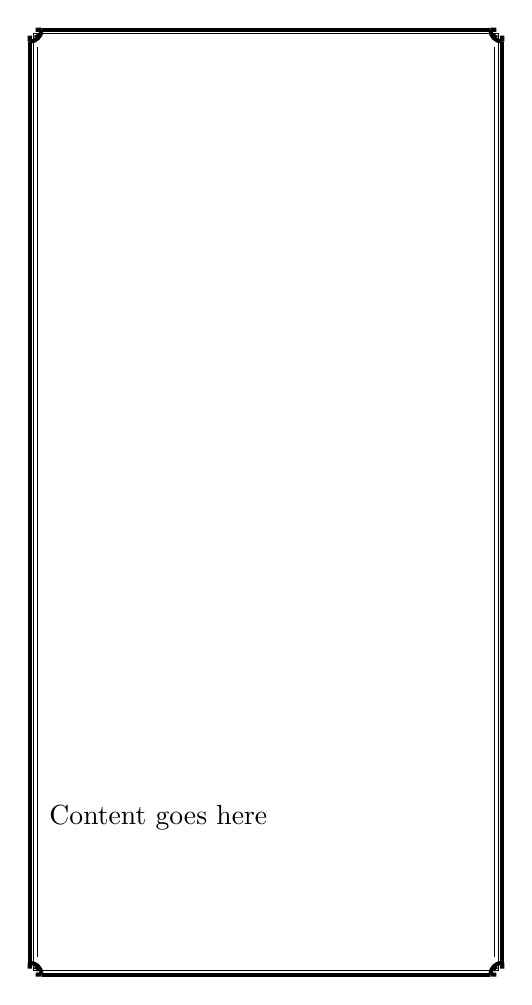
\begin{tikzpicture}
  \dndbox{0}{0}{6cm}{12cm}
  \node[text width=5.5cm, align=left] at (3, 2) {Content goes here};
\end{tikzpicture}

\end{document}


OK, let's start with a latex macro to create boxes with decorations, as are use for proficiencies, equipment, and so on.  The macro should be suitable to use inside a tikzpicture environment, using tikz, and it should take these parameters: the coordinates of the lower-left corner, and the width and height of the box.  Organize the parameters in whatever way makes the implementation simple.

Please be sure to reproduce these two aspects of the example: the mix of heavy and light rules, and the fancy corners.


Excellent!  As our next step, please define a utility {\LaTeX}
environment \begin{dndsection} for setting up a section.  It should take the same parameters as the \dndbox macro, and in addition it should take a title and a background color.   That environment should do the following:

  - Place a decorative box of the requested size at the requested location
  - Set the given background color inside the box
  - Place the title centered at the bottom, as in the examples
  - Set up a minipage environment for typesetting inside the box.

Leave a small margin between the minipage and the edges of the box, as shown in the example.

Note that the size of the box should be independent of the eventual height of the minipage.  Making things fit is the job of the user, not the environment.

Once you've done that, use your dndsection environment to define environments for each of the following sections:
attacks, magic, features, equipment, and proficiencies.

Finally, emit a sample page with all these sections, so I can test things.




\colorlet{stats}{blue!10!white}
\colorlet{proficiencies}{yellow!12!white}
\colorlet{attacks}{orange!25!white}
\colorlet{magic}{red!12!white}
\colorlet{mypurple}{red!40!blue}
\colorlet{feats}{magenta!16}
\colorlet{playername}{green!90!yellow!8!white}
\colorlet{teal}{blue!40!green}
\colorlet{equipment}{playername}


You're getting there.  That overlay option is no good.  Try these changes:

  - Explicitly give the dimensions of the tikzpicture as \textwidth, \textheight.  No other options to the tikzpicture environment.
  - Correct the section widths by using the widths in my original example
  - Place the sections at the locations originally used in the example, even though that will likely leave some blank space on the page


OK, I've done some geometry for you.  But eventually I'm going to need
two versions, one for casters and one for noncasters.  Let's talk
parameter:

  - \rightx is the X coordinate of the right column, the same for both sheets
  - Similarly for \rightwidth and \leftwidth
  - Y coordinates and heights are going to vary between casters and noncasters

For now, let's handle this by creating boolean flag \ifcaster, and use
that to control the geometries of sections as needed.

Please extract the geometries from the code I'm about to paste, and
please also use the alternate geometries in comments where available,
according to \ifcaster.  Then redo the example using \castertrue.

As noted, you'll also need to use the geometry package with a margin
of 7mm.

Finally, correct the internal minipage environments so (1) there is a
some space between them and the containing box, and (2) the text
appears at the top of the box, not the bottom.

